\newslide{Mountain Rescue Intervention}{
	\begin{block}{}
		\begin{tikzpicture}
			\node [text width=7.5cm] (lista) {
			\vspace{2.5cm}
			\begin{itemize}
				\item Call from witnesses or hikers in danger
				\item Helicopter mission
				\item {\color{blue}Evaluation of critical risk}
				\item Searching on avalanche surface
				\item Searching for ARTVA signal presence
				\item {\color{red}Fine ARTVA searching}
				\item Buried extraction
			\end{itemize}};
			\node [at=(lista.north east), anchor=north west, xshift=2cm](immagine) {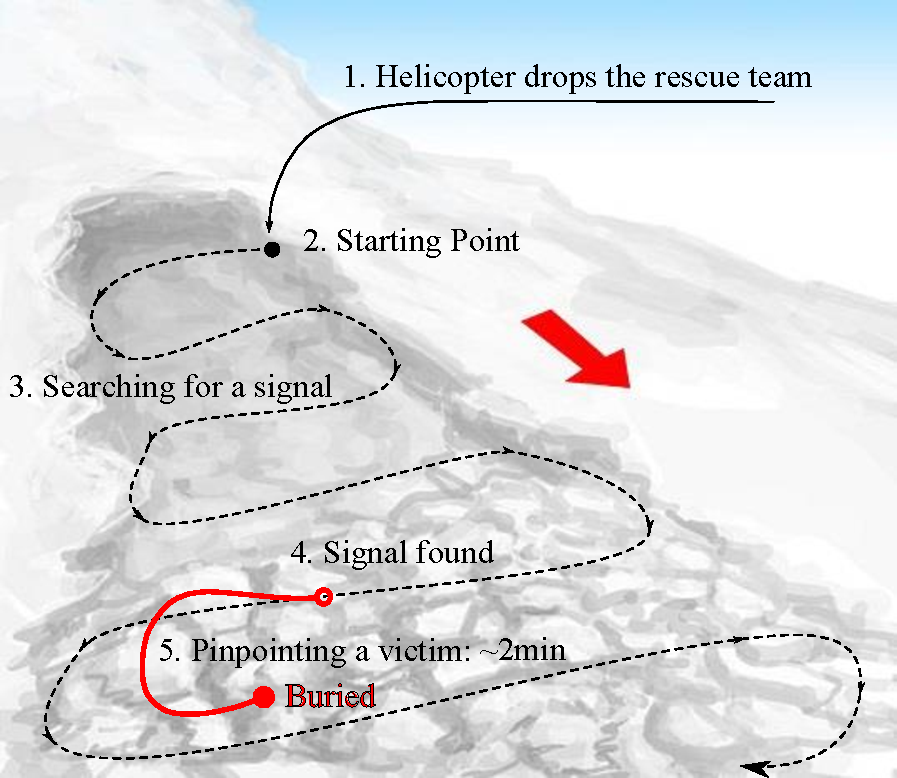
\includegraphics[scale=0.5]{img/introductive.pdf}};
			
			\node [below=of immagine,yshift=1cm] {
				\begin{tikzpicture}
					\begin{axis} [xlabel={\scriptsize Time (min)}, ylabel={\scriptsize Chances of survival (\%)},
					 enlargelimits=false, width=8cm,height=4.5cm,tick label style={font=\scriptsize}]

						\addplot [mark=none,line width=1.5] coordinates {
							(0,100)
							(15,90)
							(20,60)
							(30,50)
							(40,25)
							(120,15)
							(180,3)
						};
					\end{axis}
				\end{tikzpicture}};

		\end{tikzpicture}
	\end{block}
}

